\chapter{FPGA\label{FPGA}}
As briefly mentioned in the introduction, FPGAs consisting of an array of logic
gates. In this section we will give an overview about how they and other the
other components work and what different ways there are to configure these
chips. Modern FPGAs may also include a number of other components, for example
processors and multipliers though we will not cover those.

\section{Components}
\subsection{Lookup tables}

In boolean algebra we can represent a function as a truth table of size $2^N$
where $N$ is the amount of variables in the function. This translates directly
to binary and because of this property FPGAs extensively use lookup
tables(LUT). The way LUTs are implemented are using $N:1$ multiplexers and
$N$-bits of memory, it stores all the answers of the LUT in memory. Then the
multiplexer takes $N$ inputs and maps it to the LUTs answer. For example if we
have the following function.

$$A + B \times C$$

There are $2^3 = 8$ different answers to the function. We then
store all of these answers in memory in a table as similar to what is seen in
table \ref{tab:example_truth_table}.

\begin{table}[ht]
    \centering
    \begin{tabular}{|l|l|l|l|}
        \hline
        A & B & C & Out \\ \hline
        0 & 0 & 0 & 0   \\ \hline
        0 & 0 & 1 & 1   \\ \hline
        0 & 1 & 0 & 0   \\ \hline
        0 & 1 & 1 & 1   \\ \hline
        1 & 0 & 0 & 0   \\ \hline
        1 & 0 & 1 & 1   \\ \hline
        1 & 1 & 0 & 1   \\ \hline
        1 & 1 & 1 & 1   \\ \hline
    \end{tabular}
    \caption{Example truth table}
    \label{tab:example_truth_table}
\end{table}

% flip flops
This alone isn't enough to be able to implement everything as we cannot store
state. What we need is some way to store information, this is where delay(D)
flip-flops come in. Here we have an example of how an FPGA might use a
flip-flop as seen in Figure \ref{fig:lut_flipflop}. They can store a single bit of data, with
this the chip can store state and is now complete.

\begin{figure}[H]
    \centering
    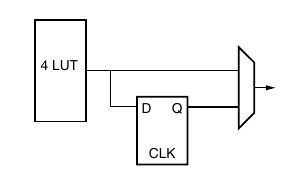
\includegraphics[scale=0.6]{lookup_table_flipflop.png}
    \caption{An example of how a lookup table could be implemented \cite{m_d_mano_digital_2012}}
    \label{fig:lut_flipflop}
\end{figure}

These LUTs are what allow for FPGAs to be reconfigured. By simply writing to
the tables the correct values it allows the chip to implement any function.
There's been studies done about how many LUTs a logic block should contain, if
there were more LUTs it would allow for more complex logic. Though adding more
inputs would also make the chip slower \cite{amano_principles_2018}.

\begin{figure}[H]
    \centering
    \label{fig:fpga_structure}
    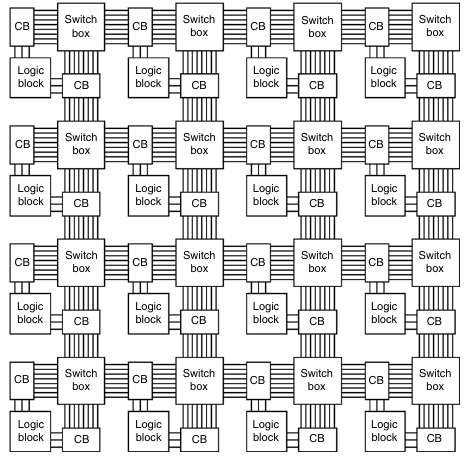
\includegraphics[scale=0.7]{fpga_structure.png}
    \caption{An example of an island-style FPGA\cite{m_d_mano_digital_2012}}
\end{figure}

\subsection{Input/Output blocks}
Input/Output blocks (I/O blocks, IOB) are blocks that are placed around the
periphery of the FPGA. They control the interface between the FPGA and external
circuits such as the clock and power usage.

\subsection{Connection block}
Along the wires by the logic blocks there are connection blocks (CB). These blocks
control which data goes into and out of a logic block. They also connect the
I/O blocks to the FPGA.

\subsection{Switch block}
A switch block (switch box, SB) is a type of block that exists at every
intersection in the wiring. As the name suggests it's built from a bunch of
switches and it's job is to route the electricity between the logic blocks.
There are different types of implementations for switch blocks, depending on
the type it will have different levels of connectivity and efficiency. Though
the specifics of this is out of the scope of this paper.

\subsection{Connections}
There are multiple ways the logic blocks can be connected, Xilinx FPGAs have
four different types of interconnects: long lines, hex lines, double lines and
direct lines. The direct lines are to connect neighboring logic gates for fast
transfer. Hex and double lines connect logic gates that are a medium length
away. Long lines go along the entire chip and are often used for signals that
everything needs to know.


\section{Configuration}
There are various ways reprogrammability can be implemented, though we're only
going to focus on the three main technologies: static RAM, flash memory and
antifuse.

\subsection{Static RAM}
Static RAM, or SRAM is a very common way to handle configuration. It's great
because it is fast and has infinite reconfiguration. The issues with SRAM is
that it's volatile which means that if power is lost so is the configuration.
Another issue is power consumption, as the SRAM cell contains 6-12 transistors
compared to flash memory which only requires roughly two transistors
\cite{amano_principles_2018}.

\subsection{Flash memory}
Flash memory is a way to store the configuration in memory without needing
power for the chip to remember it. It works by having electrically erasable
programmable read-only memory, it's benefit is that the configuration can be
remembered even if the device is powered off. The downside is that there's only
a limited amount of writes before it fails and that flash is often slower at
writing than SRAM \cite{m_d_mano_digital_2012}.

\subsection{Antifuse}
An antifuse is the opposite of a fuse, it works by having high resistance and
not allowing electricity to pass until the fuse is blown. This technology is
very reliable and rarely corrupts, which is why it's often used in places with
for example radiation. The down side of antifuses is that it can only be
programmed once, after it's programmed the fuses are blown and can not be
restored.
